% Options for packages loaded elsewhere
\PassOptionsToPackage{unicode}{hyperref}
\PassOptionsToPackage{hyphens}{url}
\PassOptionsToPackage{dvipsnames,svgnames,x11names}{xcolor}
%
\documentclass[
  letterpaper,
  DIV=11,
  numbers=noendperiod]{scrartcl}

\usepackage{amsmath,amssymb}
\usepackage{iftex}
\ifPDFTeX
  \usepackage[T1]{fontenc}
  \usepackage[utf8]{inputenc}
  \usepackage{textcomp} % provide euro and other symbols
\else % if luatex or xetex
  \usepackage{unicode-math}
  \defaultfontfeatures{Scale=MatchLowercase}
  \defaultfontfeatures[\rmfamily]{Ligatures=TeX,Scale=1}
\fi
\usepackage{lmodern}
\ifPDFTeX\else  
    % xetex/luatex font selection
\fi
% Use upquote if available, for straight quotes in verbatim environments
\IfFileExists{upquote.sty}{\usepackage{upquote}}{}
\IfFileExists{microtype.sty}{% use microtype if available
  \usepackage[]{microtype}
  \UseMicrotypeSet[protrusion]{basicmath} % disable protrusion for tt fonts
}{}
\makeatletter
\@ifundefined{KOMAClassName}{% if non-KOMA class
  \IfFileExists{parskip.sty}{%
    \usepackage{parskip}
  }{% else
    \setlength{\parindent}{0pt}
    \setlength{\parskip}{6pt plus 2pt minus 1pt}}
}{% if KOMA class
  \KOMAoptions{parskip=half}}
\makeatother
\usepackage{xcolor}
\setlength{\emergencystretch}{3em} % prevent overfull lines
\setcounter{secnumdepth}{-\maxdimen} % remove section numbering
% Make \paragraph and \subparagraph free-standing
\ifx\paragraph\undefined\else
  \let\oldparagraph\paragraph
  \renewcommand{\paragraph}[1]{\oldparagraph{#1}\mbox{}}
\fi
\ifx\subparagraph\undefined\else
  \let\oldsubparagraph\subparagraph
  \renewcommand{\subparagraph}[1]{\oldsubparagraph{#1}\mbox{}}
\fi

\usepackage{color}
\usepackage{fancyvrb}
\newcommand{\VerbBar}{|}
\newcommand{\VERB}{\Verb[commandchars=\\\{\}]}
\DefineVerbatimEnvironment{Highlighting}{Verbatim}{commandchars=\\\{\}}
% Add ',fontsize=\small' for more characters per line
\usepackage{framed}
\definecolor{shadecolor}{RGB}{241,243,245}
\newenvironment{Shaded}{\begin{snugshade}}{\end{snugshade}}
\newcommand{\AlertTok}[1]{\textcolor[rgb]{0.68,0.00,0.00}{#1}}
\newcommand{\AnnotationTok}[1]{\textcolor[rgb]{0.37,0.37,0.37}{#1}}
\newcommand{\AttributeTok}[1]{\textcolor[rgb]{0.40,0.45,0.13}{#1}}
\newcommand{\BaseNTok}[1]{\textcolor[rgb]{0.68,0.00,0.00}{#1}}
\newcommand{\BuiltInTok}[1]{\textcolor[rgb]{0.00,0.23,0.31}{#1}}
\newcommand{\CharTok}[1]{\textcolor[rgb]{0.13,0.47,0.30}{#1}}
\newcommand{\CommentTok}[1]{\textcolor[rgb]{0.37,0.37,0.37}{#1}}
\newcommand{\CommentVarTok}[1]{\textcolor[rgb]{0.37,0.37,0.37}{\textit{#1}}}
\newcommand{\ConstantTok}[1]{\textcolor[rgb]{0.56,0.35,0.01}{#1}}
\newcommand{\ControlFlowTok}[1]{\textcolor[rgb]{0.00,0.23,0.31}{#1}}
\newcommand{\DataTypeTok}[1]{\textcolor[rgb]{0.68,0.00,0.00}{#1}}
\newcommand{\DecValTok}[1]{\textcolor[rgb]{0.68,0.00,0.00}{#1}}
\newcommand{\DocumentationTok}[1]{\textcolor[rgb]{0.37,0.37,0.37}{\textit{#1}}}
\newcommand{\ErrorTok}[1]{\textcolor[rgb]{0.68,0.00,0.00}{#1}}
\newcommand{\ExtensionTok}[1]{\textcolor[rgb]{0.00,0.23,0.31}{#1}}
\newcommand{\FloatTok}[1]{\textcolor[rgb]{0.68,0.00,0.00}{#1}}
\newcommand{\FunctionTok}[1]{\textcolor[rgb]{0.28,0.35,0.67}{#1}}
\newcommand{\ImportTok}[1]{\textcolor[rgb]{0.00,0.46,0.62}{#1}}
\newcommand{\InformationTok}[1]{\textcolor[rgb]{0.37,0.37,0.37}{#1}}
\newcommand{\KeywordTok}[1]{\textcolor[rgb]{0.00,0.23,0.31}{#1}}
\newcommand{\NormalTok}[1]{\textcolor[rgb]{0.00,0.23,0.31}{#1}}
\newcommand{\OperatorTok}[1]{\textcolor[rgb]{0.37,0.37,0.37}{#1}}
\newcommand{\OtherTok}[1]{\textcolor[rgb]{0.00,0.23,0.31}{#1}}
\newcommand{\PreprocessorTok}[1]{\textcolor[rgb]{0.68,0.00,0.00}{#1}}
\newcommand{\RegionMarkerTok}[1]{\textcolor[rgb]{0.00,0.23,0.31}{#1}}
\newcommand{\SpecialCharTok}[1]{\textcolor[rgb]{0.37,0.37,0.37}{#1}}
\newcommand{\SpecialStringTok}[1]{\textcolor[rgb]{0.13,0.47,0.30}{#1}}
\newcommand{\StringTok}[1]{\textcolor[rgb]{0.13,0.47,0.30}{#1}}
\newcommand{\VariableTok}[1]{\textcolor[rgb]{0.07,0.07,0.07}{#1}}
\newcommand{\VerbatimStringTok}[1]{\textcolor[rgb]{0.13,0.47,0.30}{#1}}
\newcommand{\WarningTok}[1]{\textcolor[rgb]{0.37,0.37,0.37}{\textit{#1}}}

\providecommand{\tightlist}{%
  \setlength{\itemsep}{0pt}\setlength{\parskip}{0pt}}\usepackage{longtable,booktabs,array}
\usepackage{calc} % for calculating minipage widths
% Correct order of tables after \paragraph or \subparagraph
\usepackage{etoolbox}
\makeatletter
\patchcmd\longtable{\par}{\if@noskipsec\mbox{}\fi\par}{}{}
\makeatother
% Allow footnotes in longtable head/foot
\IfFileExists{footnotehyper.sty}{\usepackage{footnotehyper}}{\usepackage{footnote}}
\makesavenoteenv{longtable}
\usepackage{graphicx}
\makeatletter
\def\maxwidth{\ifdim\Gin@nat@width>\linewidth\linewidth\else\Gin@nat@width\fi}
\def\maxheight{\ifdim\Gin@nat@height>\textheight\textheight\else\Gin@nat@height\fi}
\makeatother
% Scale images if necessary, so that they will not overflow the page
% margins by default, and it is still possible to overwrite the defaults
% using explicit options in \includegraphics[width, height, ...]{}
\setkeys{Gin}{width=\maxwidth,height=\maxheight,keepaspectratio}
% Set default figure placement to htbp
\makeatletter
\def\fps@figure{htbp}
\makeatother
% definitions for citeproc citations
\NewDocumentCommand\citeproctext{}{}
\NewDocumentCommand\citeproc{mm}{%
  \begingroup\def\citeproctext{#2}\cite{#1}\endgroup}
\makeatletter
 % allow citations to break across lines
 \let\@cite@ofmt\@firstofone
 % avoid brackets around text for \cite:
 \def\@biblabel#1{}
 \def\@cite#1#2{{#1\if@tempswa , #2\fi}}
\makeatother
\newlength{\cslhangindent}
\setlength{\cslhangindent}{1.5em}
\newlength{\csllabelwidth}
\setlength{\csllabelwidth}{3em}
\newenvironment{CSLReferences}[2] % #1 hanging-indent, #2 entry-spacing
 {\begin{list}{}{%
  \setlength{\itemindent}{0pt}
  \setlength{\leftmargin}{0pt}
  \setlength{\parsep}{0pt}
  % turn on hanging indent if param 1 is 1
  \ifodd #1
   \setlength{\leftmargin}{\cslhangindent}
   \setlength{\itemindent}{-1\cslhangindent}
  \fi
  % set entry spacing
  \setlength{\itemsep}{#2\baselineskip}}}
 {\end{list}}
\usepackage{calc}
\newcommand{\CSLBlock}[1]{\hfill\break\parbox[t]{\linewidth}{\strut\ignorespaces#1\strut}}
\newcommand{\CSLLeftMargin}[1]{\parbox[t]{\csllabelwidth}{\strut#1\strut}}
\newcommand{\CSLRightInline}[1]{\parbox[t]{\linewidth - \csllabelwidth}{\strut#1\strut}}
\newcommand{\CSLIndent}[1]{\hspace{\cslhangindent}#1}

\KOMAoption{captions}{tableheading}
\makeatletter
\@ifpackageloaded{caption}{}{\usepackage{caption}}
\AtBeginDocument{%
\ifdefined\contentsname
  \renewcommand*\contentsname{Table of contents}
\else
  \newcommand\contentsname{Table of contents}
\fi
\ifdefined\listfigurename
  \renewcommand*\listfigurename{List of Figures}
\else
  \newcommand\listfigurename{List of Figures}
\fi
\ifdefined\listtablename
  \renewcommand*\listtablename{List of Tables}
\else
  \newcommand\listtablename{List of Tables}
\fi
\ifdefined\figurename
  \renewcommand*\figurename{Figure}
\else
  \newcommand\figurename{Figure}
\fi
\ifdefined\tablename
  \renewcommand*\tablename{Table}
\else
  \newcommand\tablename{Table}
\fi
}
\@ifpackageloaded{float}{}{\usepackage{float}}
\floatstyle{ruled}
\@ifundefined{c@chapter}{\newfloat{codelisting}{h}{lop}}{\newfloat{codelisting}{h}{lop}[chapter]}
\floatname{codelisting}{Listing}
\newcommand*\listoflistings{\listof{codelisting}{List of Listings}}
\makeatother
\makeatletter
\makeatother
\makeatletter
\@ifpackageloaded{caption}{}{\usepackage{caption}}
\@ifpackageloaded{subcaption}{}{\usepackage{subcaption}}
\makeatother
\ifLuaTeX
  \usepackage{selnolig}  % disable illegal ligatures
\fi
\usepackage{bookmark}

\IfFileExists{xurl.sty}{\usepackage{xurl}}{} % add URL line breaks if available
\urlstyle{same} % disable monospaced font for URLs
\hypersetup{
  pdftitle={Mapping Childhood Vulnerability in New South Wales},
  pdfauthor={Mu},
  colorlinks=true,
  linkcolor={blue},
  filecolor={Maroon},
  citecolor={Blue},
  urlcolor={Blue},
  pdfcreator={LaTeX via pandoc}}

\title{Mapping Childhood Vulnerability in New South Wales}
\usepackage{etoolbox}
\makeatletter
\providecommand{\subtitle}[1]{% add subtitle to \maketitle
  \apptocmd{\@title}{\par {\large #1 \par}}{}{}
}
\makeatother
\subtitle{Variable Definitions and Geographic Visualization}
\author{Mu}
\date{2024-08-26}

\begin{document}
\maketitle

\renewcommand*\contentsname{Table of contents}
{
\hypersetup{linkcolor=}
\setcounter{tocdepth}{3}
\tableofcontents
}
\section{Introduction}\label{introduction}

This document provides an overview of the maps and variable definitions
used in analyzing early childhood vulnerability in Australia. The data
utilized in these maps are derived from model-based estimations applied
to the Australia Early Childhood Development Census (AEDC) data(AEDC
2024). The model borrow the strength from socio-economic indexes for
areas (SEIFA) and the Accessibility/Remoteness Index of Australia (ARIA)
to estimate the proportion of children in each Statistical Area Level 3
(SA3) who are developmentally vulnerable in each of five domains of the
AEDC (Baffour et al. 2024).

We also show the data of indigenous population in each SA3 region which
provided by the Australian Bureau of Statistics (ABS) via
TableBuilder(ABS 2021). We use the ASGS16 SA3 shape file to map the
proportion of children developmentally vulnerable in each domain across
New South Wales. The SA3 shape file is available from the Australian
Bureau of Statistics (ABS) website(ABS 2016).

\section{Variable definitions}\label{variable-definitions}

We use the following variables in our data file
\texttt{Input/data\_AEDC.csv}.

\begin{itemize}
\tightlist
\item
  \texttt{variable}: name of domains of indicators of early childhood
  vulnerability, which are:

  \begin{itemize}
  \tightlist
  \item
    \texttt{Health}: Physical Health and Wellbeing
  \item
    \texttt{Social}: Social Competence
  \item
    \texttt{Emotional}: Emotional Maturity
  \item
    \texttt{Language}: Language and Cognitive Skills
  \item
    \texttt{Communication}: Communication Skills and General Knowledge
  \end{itemize}
\item
  \texttt{model}: name of the model used to estimate the proportion of
  children developmentally vulnerable in each domain. Here we use
  \texttt{M4} model as this was found to have the best performance in
  the study(Baffour et al. 2024).
\item
  \texttt{SA3\_NAME16}: Official name of SA3 region
\item
  \texttt{SA4\_NAME16}: Official name of SA4 region
\item
  \texttt{GCC\_NAME16}: Official name of Greater Capital City region
\item
  \texttt{state}: State or Territory in which the SA3 region is located
\item
  \texttt{IRSD}: Index of Relative Socio-economic Disadvantage (IRSD)
  score
\item
  \texttt{ARIA}: Accessibility/Remoteness Index of Australia (ARIA)
  score
\item
  \texttt{vulnerble\_count}: Number of children developmentally
  vulnerable in the SA3
\item
  \texttt{sample\_size}: Number of children in AEDC in the SA3
\item
  \texttt{vulnerable\_rate}: Proportion of children developmentally
  vulnerable in the SA3
\item
  \texttt{vulnerable\_rate\_model}: Proportion of children
  developmentally vulnerable in the SA3 estimated by the model
\item
  \texttt{indig\_yes}: number of people who identify as Indigenous in
  the SA3
\item
  \texttt{indig\_no}: number of people who do not identify as Indigenous
  in the SA3
\item
  \texttt{indig\_not\_stated}: number of people who did not state their
  Indigenous status in the SA3
\item
  \texttt{indig\_rate}: Proportion of people who identify as Indigenous
  in the SA3
\item
  \texttt{usual\_resident\_population}: Number of usual residents in the
  SA3
\end{itemize}

\section{Mapping in NSW}\label{mapping-in-nsw}

We use the \texttt{spdep} package to read the shape file and the
\texttt{ggplot2} package to create the maps. We use the \texttt{ggpubr}
package to combine the maps into a single figure.

\subsection{Mapping Vulnerability
Levels}\label{mapping-vulnerability-levels}

Here the map shows the proportion of children developmentally vulnerable
in each domain across New South Wales and Greater Sydney. The maps are
color-coded by deciles of vulnerability levels, with red indicating
higher vulnerability and green indicating lower vulnerability.

\begin{Shaded}
\begin{Highlighting}[]
\NormalTok{FUN\_Mapping }\OtherTok{\textless{}{-}} \ControlFlowTok{function}\NormalTok{(Variable, FullName)\{}
  
\NormalTok{  p1 }\OtherTok{\textless{}{-}}\NormalTok{ dat\_map }\SpecialCharTok{\%\textgreater{}\%}
    \FunctionTok{filter}\NormalTok{(variable }\SpecialCharTok{==}\NormalTok{ Variable) }\SpecialCharTok{\%\textgreater{}\%}
    \FunctionTok{ggplot}\NormalTok{() }\SpecialCharTok{+}
    \FunctionTok{geom\_sf}\NormalTok{(}\FunctionTok{aes}\NormalTok{(}\AttributeTok{fill =}\NormalTok{ vulnerable\_rate\_model\_cat),}
            \AttributeTok{color =} \StringTok{"black"}\NormalTok{) }\SpecialCharTok{+}
    \FunctionTok{scale\_fill\_brewer}\NormalTok{(}\AttributeTok{palette =} \StringTok{"RdYlGn"}\NormalTok{,}
                      \AttributeTok{direction =} \SpecialCharTok{{-}}\DecValTok{1}\NormalTok{,}
                      \AttributeTok{na.value =} \StringTok{"grey"}\NormalTok{) }\SpecialCharTok{+} 
    \FunctionTok{labs}\NormalTok{(}\AttributeTok{title =} \StringTok{"New South Wales"}\NormalTok{,}
         \AttributeTok{fill =} \StringTok{"Vulnerability Levels (Deciles)"}\NormalTok{) }\SpecialCharTok{+}
    \FunctionTok{theme\_void}\NormalTok{() }\SpecialCharTok{+}
    \FunctionTok{theme}\NormalTok{(}\AttributeTok{plot.title =} \FunctionTok{element\_text}\NormalTok{(}\AttributeTok{hjust =} \FloatTok{0.5}\NormalTok{,}
                                    \AttributeTok{size =} \DecValTok{12}\NormalTok{))}
  
\NormalTok{  p2 }\OtherTok{\textless{}{-}}\NormalTok{ dat\_map }\SpecialCharTok{\%\textgreater{}\%}
    \FunctionTok{filter}\NormalTok{(variable }\SpecialCharTok{==}\NormalTok{ Variable,}
\NormalTok{           GCC\_NAME16 }\SpecialCharTok{==} \StringTok{"Greater Sydney"}\NormalTok{) }\SpecialCharTok{\%\textgreater{}\%}
    \FunctionTok{ggplot}\NormalTok{() }\SpecialCharTok{+}
    \FunctionTok{geom\_sf}\NormalTok{(}\FunctionTok{aes}\NormalTok{(}\AttributeTok{fill =}\NormalTok{ vulnerable\_rate\_model\_cat),}
            \AttributeTok{color =} \StringTok{"black"}\NormalTok{) }\SpecialCharTok{+}
    \FunctionTok{scale\_fill\_brewer}\NormalTok{(}\AttributeTok{palette =} \StringTok{"RdYlGn"}\NormalTok{,}
                      \AttributeTok{direction =} \SpecialCharTok{{-}}\DecValTok{1}\NormalTok{,}
                      \AttributeTok{na.value =} \StringTok{"grey"}\NormalTok{) }\SpecialCharTok{+} 
    \FunctionTok{labs}\NormalTok{(}\AttributeTok{title =} \StringTok{"Greater Sydney"}\NormalTok{,}
         \AttributeTok{fill =} \StringTok{"Vulnerability Levels (Deciles)"}\NormalTok{) }\SpecialCharTok{+}
    \FunctionTok{theme\_void}\NormalTok{() }\SpecialCharTok{+}
    \FunctionTok{theme}\NormalTok{(}\AttributeTok{plot.title =} \FunctionTok{element\_text}\NormalTok{(}\AttributeTok{hjust =} \FloatTok{0.5}\NormalTok{,}
                                    \AttributeTok{size =} \DecValTok{12}\NormalTok{))}
  
\NormalTok{  map }\OtherTok{\textless{}{-}} \FunctionTok{ggarrange}\NormalTok{(}\AttributeTok{plotlist =} \FunctionTok{list}\NormalTok{(p1, p2),}
                   \AttributeTok{ncol =} \DecValTok{2}\NormalTok{,}
                   \AttributeTok{common.legend =} \ConstantTok{TRUE}\NormalTok{, }\AttributeTok{legend =} \StringTok{"bottom"}\NormalTok{) }\SpecialCharTok{\%\textgreater{}\%}
    \FunctionTok{annotate\_figure}\NormalTok{(}\AttributeTok{top =} \FunctionTok{text\_grob}\NormalTok{(}\FunctionTok{str\_c}\NormalTok{(}\StringTok{"Child Developmental Vulnerability by SA3 in 2018"}\NormalTok{,}
                                          \StringTok{"}\SpecialCharTok{\textbackslash{}n}\StringTok{"}\NormalTok{, FullName), }
                                    \AttributeTok{face =} \StringTok{"bold"}\NormalTok{,}
                                    \AttributeTok{hjust =} \FloatTok{0.5}\NormalTok{,}
                                    \AttributeTok{size =} \DecValTok{14}\NormalTok{))}
  \FunctionTok{return}\NormalTok{(map)}
\NormalTok{\}}

\FunctionTok{FUN\_Mapping}\NormalTok{(}\StringTok{"Health"}\NormalTok{, }\StringTok{"Physical Health \& Wellbeing"}\NormalTok{)}
\end{Highlighting}
\end{Shaded}

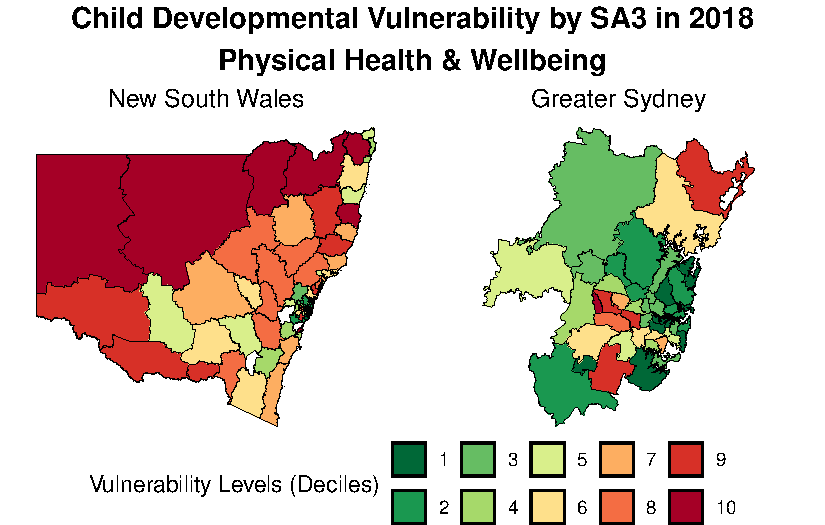
\includegraphics{variable_def_and_maps_files/figure-pdf/maps-AEDC-1.pdf}

\begin{Shaded}
\begin{Highlighting}[]
\FunctionTok{FUN\_Mapping}\NormalTok{(}\StringTok{"Social"}\NormalTok{, }\StringTok{"Social Competence"}\NormalTok{)}
\end{Highlighting}
\end{Shaded}

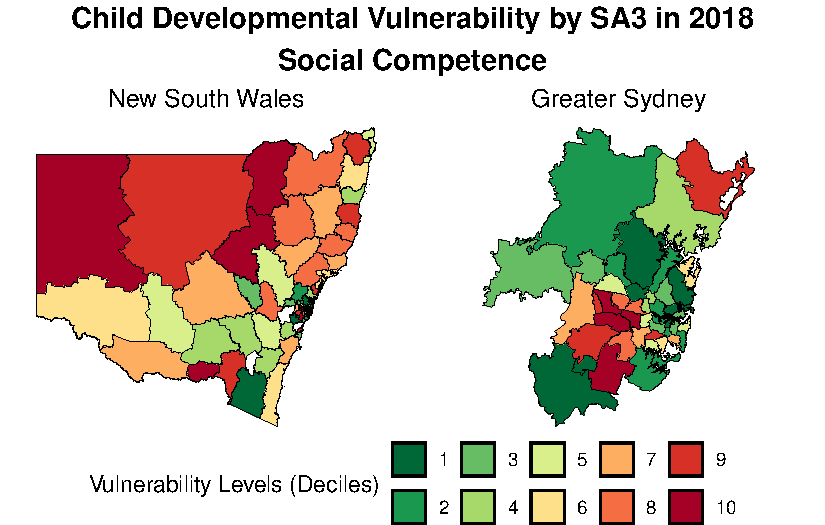
\includegraphics{variable_def_and_maps_files/figure-pdf/maps-AEDC-2.pdf}

\begin{Shaded}
\begin{Highlighting}[]
\FunctionTok{FUN\_Mapping}\NormalTok{(}\StringTok{"Emotional"}\NormalTok{, }\StringTok{"Emotional Maturity"}\NormalTok{)}
\end{Highlighting}
\end{Shaded}

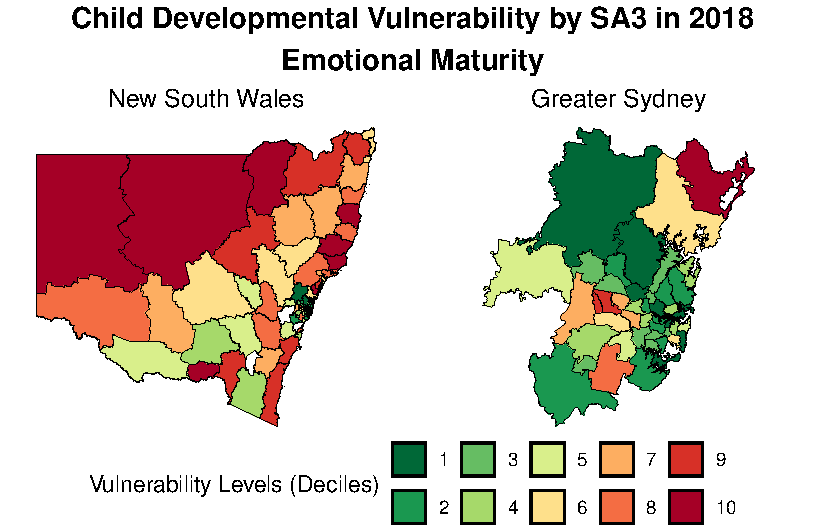
\includegraphics{variable_def_and_maps_files/figure-pdf/maps-AEDC-3.pdf}

\begin{Shaded}
\begin{Highlighting}[]
\FunctionTok{FUN\_Mapping}\NormalTok{(}\StringTok{"Language"}\NormalTok{, }\StringTok{"Language \& Cognitive Skills"}\NormalTok{)}
\end{Highlighting}
\end{Shaded}

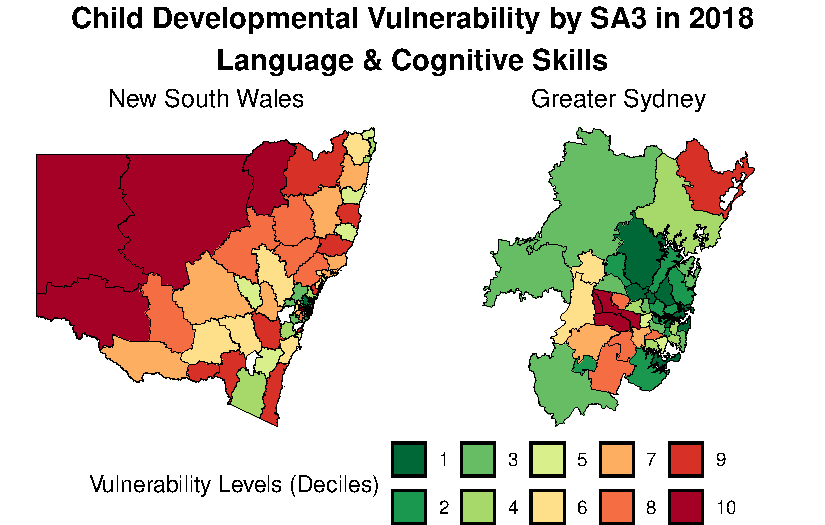
\includegraphics{variable_def_and_maps_files/figure-pdf/maps-AEDC-4.pdf}

\begin{Shaded}
\begin{Highlighting}[]
\FunctionTok{FUN\_Mapping}\NormalTok{(}\StringTok{"Communication"}\NormalTok{, }\StringTok{"Communication Skills \& General Knowledge"}\NormalTok{)}
\end{Highlighting}
\end{Shaded}

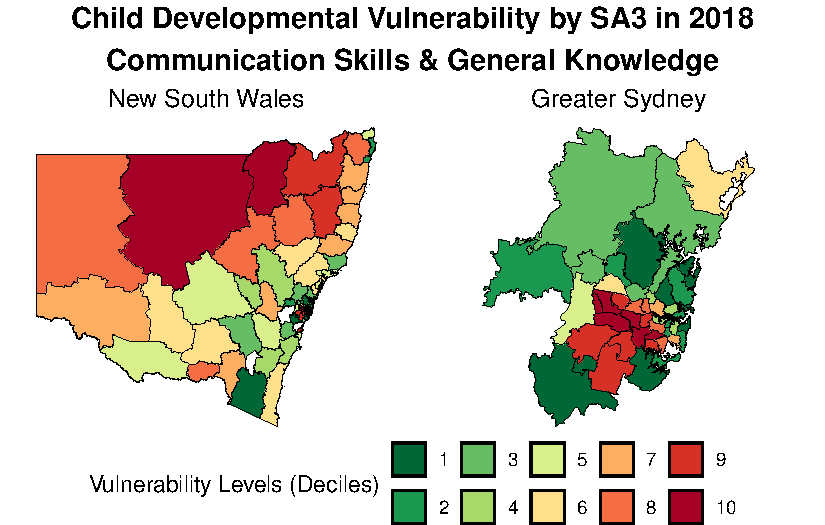
\includegraphics{variable_def_and_maps_files/figure-pdf/maps-AEDC-5.pdf}

\subsection{Mapping Proportion of Indigenous
Population}\label{mapping-proportion-of-indigenous-population}

We also provide a map showing the proportion of the Indigenous
population in New South Wales and Greater Sydney.

\begin{Shaded}
\begin{Highlighting}[]
\NormalTok{p1 }\OtherTok{\textless{}{-}}\NormalTok{ dat\_map }\SpecialCharTok{\%\textgreater{}\%}
  \FunctionTok{filter}\NormalTok{(variable }\SpecialCharTok{==} \StringTok{"Health"}\NormalTok{) }\SpecialCharTok{\%\textgreater{}\%}
  \FunctionTok{mutate}\NormalTok{(}\AttributeTok{indig\_ratio =}\NormalTok{ indig\_yes }\SpecialCharTok{/}\NormalTok{ (indig\_yes }\SpecialCharTok{+}\NormalTok{ indig\_no),}
         \AttributeTok{indig\_ratio\_cat =} \FunctionTok{factor}\NormalTok{(}\FunctionTok{ntile}\NormalTok{(indig\_ratio,}\DecValTok{10}\NormalTok{))) }\SpecialCharTok{\%\textgreater{}\%}
  \FunctionTok{ggplot}\NormalTok{() }\SpecialCharTok{+}
  \FunctionTok{geom\_sf}\NormalTok{(}\FunctionTok{aes}\NormalTok{(}\AttributeTok{fill =}\NormalTok{ indig\_ratio\_cat),}
          \AttributeTok{color =} \StringTok{"black"}\NormalTok{) }\SpecialCharTok{+}
  \FunctionTok{scale\_fill\_brewer}\NormalTok{(}\AttributeTok{palette =} \StringTok{"RdYlGn"}\NormalTok{,}
                    \AttributeTok{direction =} \SpecialCharTok{{-}}\DecValTok{1}\NormalTok{,}
                    \AttributeTok{na.value =} \StringTok{"grey"}\NormalTok{) }\SpecialCharTok{+} 
  \FunctionTok{labs}\NormalTok{(}\AttributeTok{title =} \StringTok{"New South Wales"}\NormalTok{,}
       \AttributeTok{fill =} \StringTok{"Proportion (Deciles)"}\NormalTok{) }\SpecialCharTok{+}
  \FunctionTok{theme\_void}\NormalTok{() }\SpecialCharTok{+}
  \FunctionTok{theme}\NormalTok{(}\AttributeTok{plot.title =} \FunctionTok{element\_text}\NormalTok{(}\AttributeTok{hjust =} \FloatTok{0.5}\NormalTok{,}
                                  \AttributeTok{size =} \DecValTok{12}\NormalTok{))}

\NormalTok{p2 }\OtherTok{\textless{}{-}}\NormalTok{ dat\_map }\SpecialCharTok{\%\textgreater{}\%}
  \FunctionTok{filter}\NormalTok{(variable }\SpecialCharTok{==} \StringTok{"Health"}\NormalTok{,}
\NormalTok{         GCC\_NAME16 }\SpecialCharTok{==} \StringTok{"Greater Sydney"}\NormalTok{) }\SpecialCharTok{\%\textgreater{}\%}
  \FunctionTok{mutate}\NormalTok{(}\AttributeTok{indig\_ratio =}\NormalTok{ indig\_yes }\SpecialCharTok{/}\NormalTok{ (indig\_yes }\SpecialCharTok{+}\NormalTok{ indig\_no),}
         \AttributeTok{indig\_ratio\_cat =} \FunctionTok{factor}\NormalTok{(}\FunctionTok{ntile}\NormalTok{(indig\_ratio,}\DecValTok{5}\NormalTok{))) }\SpecialCharTok{\%\textgreater{}\%}
  \FunctionTok{ggplot}\NormalTok{() }\SpecialCharTok{+}
  \FunctionTok{geom\_sf}\NormalTok{(}\FunctionTok{aes}\NormalTok{(}\AttributeTok{fill =}\NormalTok{ indig\_ratio\_cat),}
          \AttributeTok{color =} \StringTok{"black"}\NormalTok{) }\SpecialCharTok{+}
  \FunctionTok{scale\_fill\_brewer}\NormalTok{(}\AttributeTok{palette =} \StringTok{"RdYlGn"}\NormalTok{,}
                    \AttributeTok{direction =} \SpecialCharTok{{-}}\DecValTok{1}\NormalTok{,}
                    \AttributeTok{na.value =} \StringTok{"grey"}\NormalTok{) }\SpecialCharTok{+} 
  \FunctionTok{labs}\NormalTok{(}\AttributeTok{title =} \StringTok{"Greater Sydney"}\NormalTok{,}
       \AttributeTok{fill =} \StringTok{"Proportion (5 Quantiles)"}\NormalTok{) }\SpecialCharTok{+}
  \FunctionTok{theme\_void}\NormalTok{() }\SpecialCharTok{+}
  \FunctionTok{theme}\NormalTok{(}\AttributeTok{plot.title =} \FunctionTok{element\_text}\NormalTok{(}\AttributeTok{hjust =} \FloatTok{0.5}\NormalTok{,}
                                  \AttributeTok{size =} \DecValTok{12}\NormalTok{))}

\FunctionTok{ggarrange}\NormalTok{(}\AttributeTok{plotlist =} \FunctionTok{list}\NormalTok{(p1, p2),}
          \AttributeTok{ncol =} \DecValTok{2}\NormalTok{,}
          \AttributeTok{common.legend =} \ConstantTok{TRUE}\NormalTok{, }\AttributeTok{legend =} \StringTok{"bottom"}\NormalTok{) }\SpecialCharTok{\%\textgreater{}\%}
  \FunctionTok{annotate\_figure}\NormalTok{(}\AttributeTok{top =} \FunctionTok{text\_grob}\NormalTok{(}\FunctionTok{str\_c}\NormalTok{(}\StringTok{"Indigenous Population"}\NormalTok{,}
                                        \StringTok{"}\SpecialCharTok{\textbackslash{}n}\StringTok{"}\NormalTok{,  }\StringTok{"by SA3 in 2016"}\NormalTok{), }
                                  \AttributeTok{face =} \StringTok{"bold"}\NormalTok{,}
                                  \AttributeTok{hjust =} \FloatTok{0.5}\NormalTok{,}
                                  \AttributeTok{size =} \DecValTok{14}\NormalTok{))}
\end{Highlighting}
\end{Shaded}

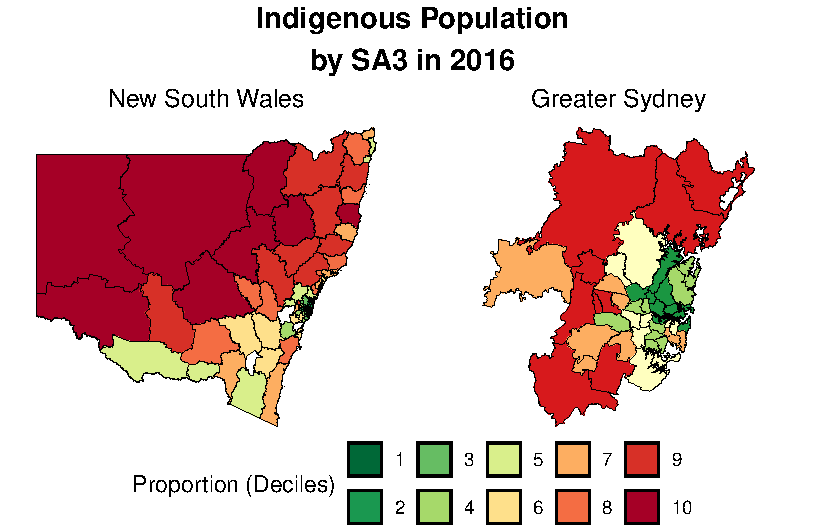
\includegraphics{variable_def_and_maps_files/figure-pdf/maps-indig-1.pdf}

\section{References}\label{references}

\phantomsection\label{refs}
\begin{CSLReferences}{1}{0}
\bibitem[\citeproctext]{ref-ASGS2016}
ABS. 2016. {``Australian Statistical Geography Standard (ASGS): Volume 1
- Main Structure and Greater Capital City Statistical Areas, July
2016.''} Australian Bureau of Statistics.
\url{https://www.abs.gov.au/ausstats/abs@.nsf/mf/1270.0.55.001}.

\bibitem[\citeproctext]{ref-ABS_TableBuilder}
---------. 2021. {``Australian Bureau of Statistics: TableBuilder.''}
Australian Bureau of Statistics.
\url{https://www.abs.gov.au/statistics/microdata-tablebuilder/tablebuilder}.

\bibitem[\citeproctext]{ref-AEDC_Data}
AEDC. 2024. {``Australian Early Development Census Data.''}
\url{https://www.aedc.gov.au/data}.

\bibitem[\citeproctext]{ref-baffour2024utility}
Baffour, Bernard, Sumonkanti Das, Mu Li, and Alice Richardson. 2024.
{``The Utility of Socioeconomic and Remoteness Indicators in
Understanding the Geographical Variation in the Regional Prevalence of
Early Childhood Vulnerability in Australia.''} \emph{Child Indicators
Research}, 1--37.

\end{CSLReferences}



\end{document}
